\section{Evaluation}
\label{sec:eval}

% These top level graphs are based on raw data and pick some select points.
% If you want to see the full tput-latency graphs, uncomment the section of graphs at the bottom

%%%%%%%%%%%%%%%%%%%%%%%%%%%%%%%%%%%%%%%%
%%%%%%%%%%%% Uniform fanout %%%%%%%%%%%%
%%%%%%%%%%%%%%%%%%%%%%%%%%%%%%%%%%%%%%%%
\begin{comment}
% Single shard p99 + p50
\begin{figure*}[!htb]
\centering
\subfloat[1 shard p99]{
  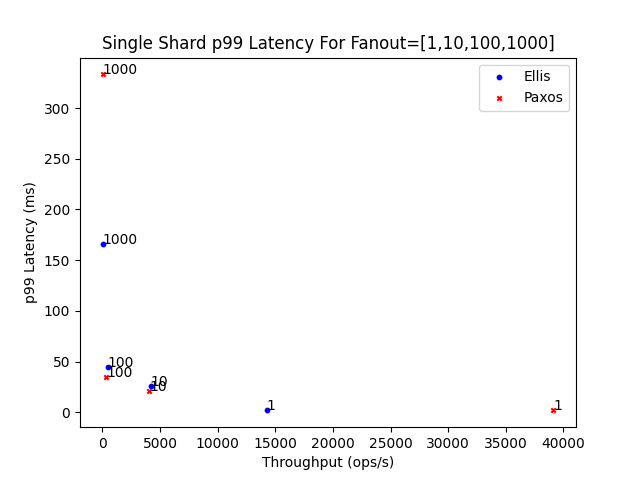
\includegraphics[scale=.6]{figs/1shardp99.png}
  \label{fig:1shardp99}
}
\subfloat[1 shard p50]{
  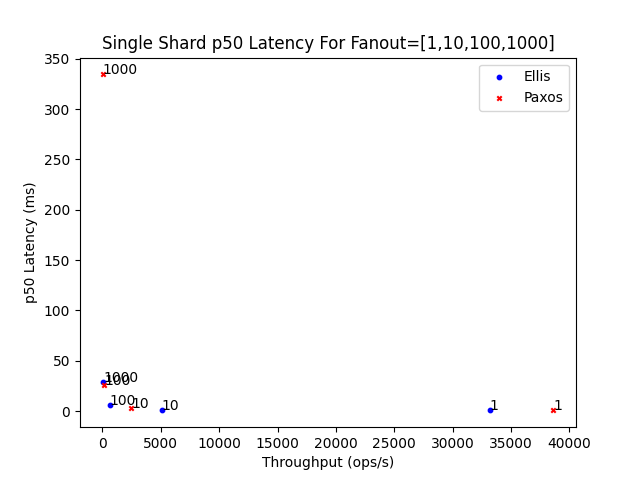
\includegraphics[scale=.6]{figs/1shardp50.png}
  \label{fig:1shardp50}
}
\hspace{0mm}
% 3 shards p99 + p50
\centering
\subfloat[3 shard p99]{
  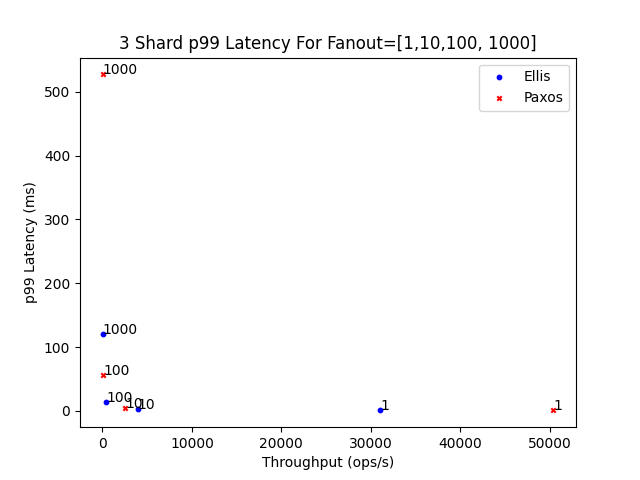
\includegraphics[scale=.6]{figs/3shardp99.png}
  \label{fig:3shardp99}
}
\subfloat[3 shard p50]{
  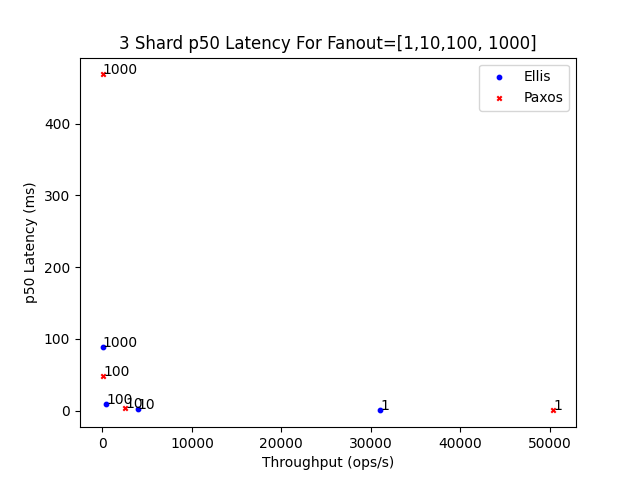
\includegraphics[scale=.6]{figs/3shardp50.png}
  \label{fig:3shardp50}
}
\hspace{0mm}
% 9 shards p99 + p50
\centering
\subfloat[9 shard p99]{
  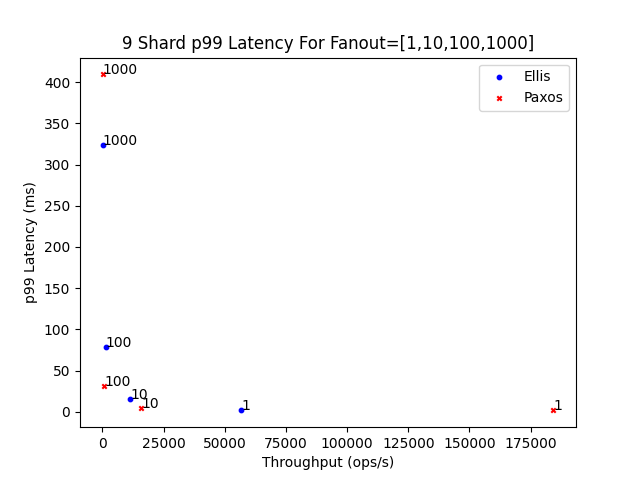
\includegraphics[scale=.6]{figs/9shardp99.png}
  \label{fig:9shardp99}
}
\subfloat[9 shard p50]{
  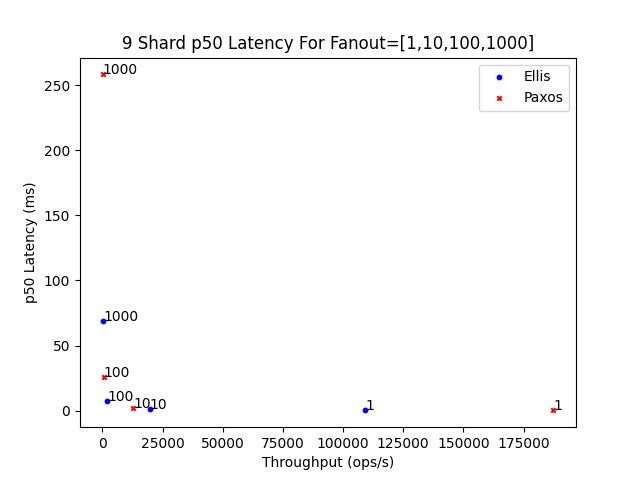
\includegraphics[scale=.6]{figs/9shardp50.png}
  \label{fig:9shardp50}
}
\caption{p99 and p50 for various shard settings.}
\end{figure*}
\end{comment}

%TODO
We evaluate \sys{}'s performance handling requests from multi-dispatch clients
compared to Multi-Paxos's performance handling requests from single-dispatch
clients.  We focus on measuring the performance (latency and throughput) of
batches of requests to evaluate the impact on end-to-end application
requests that fan out to multiple data store operations. We also evaluate how
\sys{} scales with the number of shards and how sensitive performance is to
skewed workloads.
%We report on both the p99 and p50 for application-request latency.
%We find p50 a useful metric to look at since our decision to evaluate application-level requests is already end-user facing.
We show \sys{} has lower throughput than Multi-Paxos for any particular
number of shards but reduces end-to-end latency for application-level requests
by up to 75\% when fanout increases and scales with the number of shards.

\subsection{Experimental Setup}
All experiments ran on Cloudlab's Utah platform, using
\texttt{m510} machines~\cite{duplyakin2019cloudlab}.  Each machine has 1 Intel Xeon-D processor with 8 physical cores
running at 2 GHz (hyper-threading enabled), 64 GB of DDR4-2133 RAM, and a 10
Gb/s NIC\@.  Our setup consists of a 9-node server cluster and 2 additional client machines.
The round-trip latency between all machines is 150 $\mu$s.  Each shard has three replicas,
on different physical machines. For multi-sharded experiments we place
shard leaders on separate physical machines. Clients are distributed
evenly across the client machines.

We do not consider failures in this evaluation. Failures degrade performance for
most protocols but are rare. Thus, \emph{performance} under failures is not a goal
for either \mpaxos{} or \system{}. Section~\ref{sec:design} describes how \system{}
handles failures.


% \al{combine experimental set-up and client design. get rid of metrics, workload,
% failures and replace with, approximately, one sentence each in the experimental
% setup or eval intro}

\subsection{Client Design}
Clients submit application-level requests. Each application-level request
submits $n$ (the fanout parameter for an experiment) system-level operations.

Single-dispatch clients interacting with \mpaxos{} have one in-flight operation at
a time. Multi-dispatch clients interacting with \system{} send $n$ system-level
operations concurrently, in order, waiting until all operations complete before
issuing the next batch. Both are closed-loop clients that submit a single
application-level request at a time.
In each experiment, we scale the number of clients issuing requests to both
systems from 2 to 128 by factors of 2.

% \al{idk... is it worth noting? If so, not here}
% It's worth noting that since multi-dispatch clients have $n$ requests in-flight at a time, while single-dispatch clients only have 1 request in-flight at a time, \system leaders have to deal with $n$ more requests than \mpaxos at any given time for the same number of clients.

%For a fair comparison between MDL and SDL, we keep the number of outstanding requests sent to each system the same. To achieve this, MDL uses a smaller number of clients $K$ with the specified number $N$ of outstanding requests per client, while SDL uses $K*N$ clients each with 1 outstanding request per client.

% \wl{How does keeping the overall number of requests the same mean the load is the same? We discussed this, you can explain this clearly: keep number of outstanding requests the same in both systems, for mdl this uses a smaller number of clients with the specified number of outstanding requests per client, for sdl its N clients with 1 outstanding request per client.}

%\subsection{Workload}
%We consider uniform and skewed key distributions to explore a more representative range of realistic workloads. For the latter, we generate keys according to a Zipfian distribution with varying skew values $\theta \in \{0.5, 0.7, 0.9, 1.1, 1.3\}$, and use a keyspace of size 1 million.
%
%We do not vary the request type at all, all workloads are 100\% writes, since neither our protocol nor basic Paxos implement op-type specific optimizations.

\subsection{Single-Shard}
%%%%%%%%%%%%%%%%%%%%%%%%%%%%%%%%%%%%%%%%%%%%%%%%%%%%%%%%%%%%%%%%%%%%%%%%%%%%%%%%%%%
%%%%%%%%%%%%%%%%%%%%%%%%%%%%%%%%%%%%%%%%%%%%%%%%%%%%%%%%%%%%%%%%%%%%%%%%%%%%%%%%%%%
%%%%%%%%%%%%%%%%%%%%%%%%%%%%%%%%%%%%%%%%
%%%%%%%% 1 shard uniform p99 %%%%%%%%%%%
%%%%%%%%%%%%%%%%%%%%%%%%%%%%%%%%%%%%%%%%
\begin{figure*}[tbp]
\centering
\subfloat[Fanout\xspace1]{
  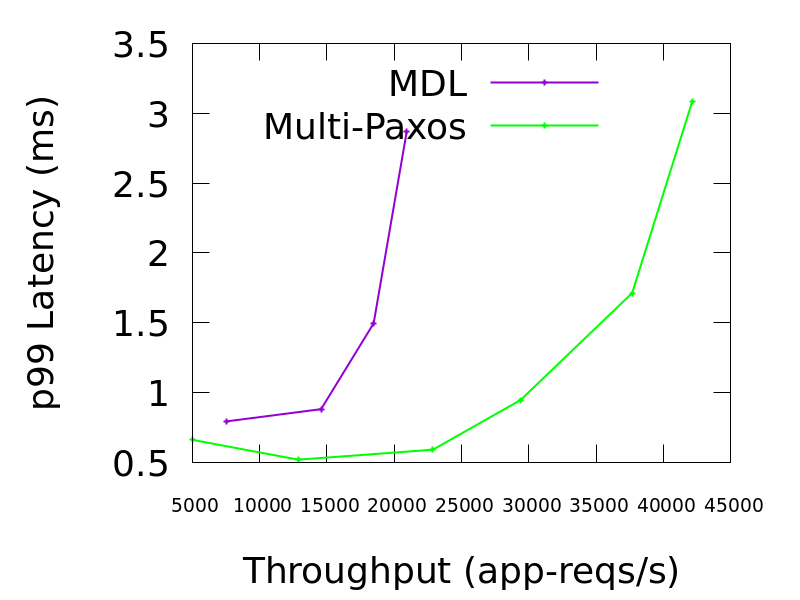
\includegraphics[scale=.15]{figs/1sh_f1_p99.png}
  \label{fig:1shardp99first}
}
\subfloat[Fanout\xspace10]{
  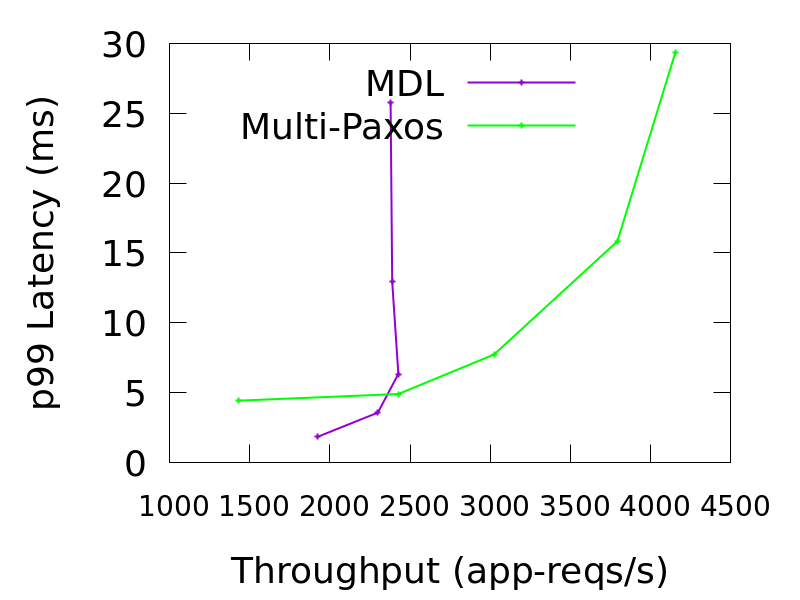
\includegraphics[scale=.15]{figs/1sh_f10_p99.png}
}
%\hspace{0mm}
\subfloat[Fanout\xspace100]{
  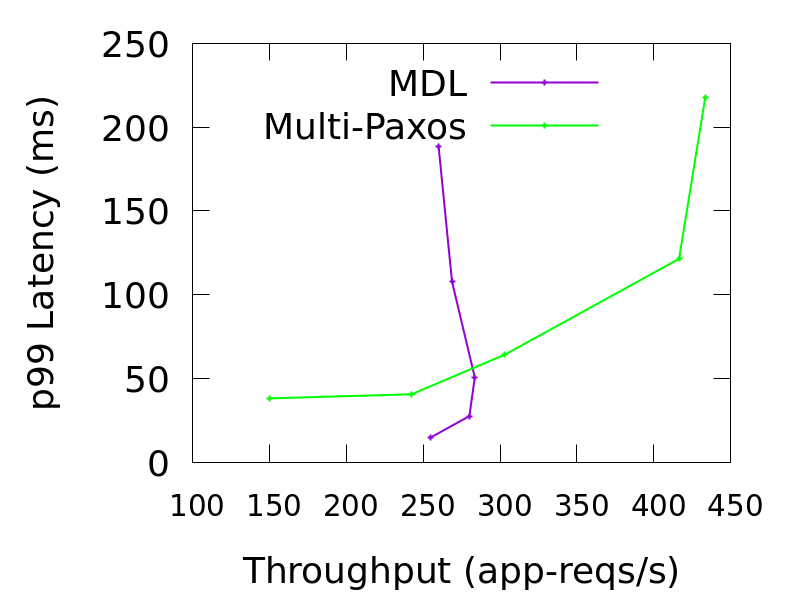
\includegraphics[scale=.15]{figs/1sh_f100_p99.png}
}
\subfloat[Fanout\xspace1000]{
  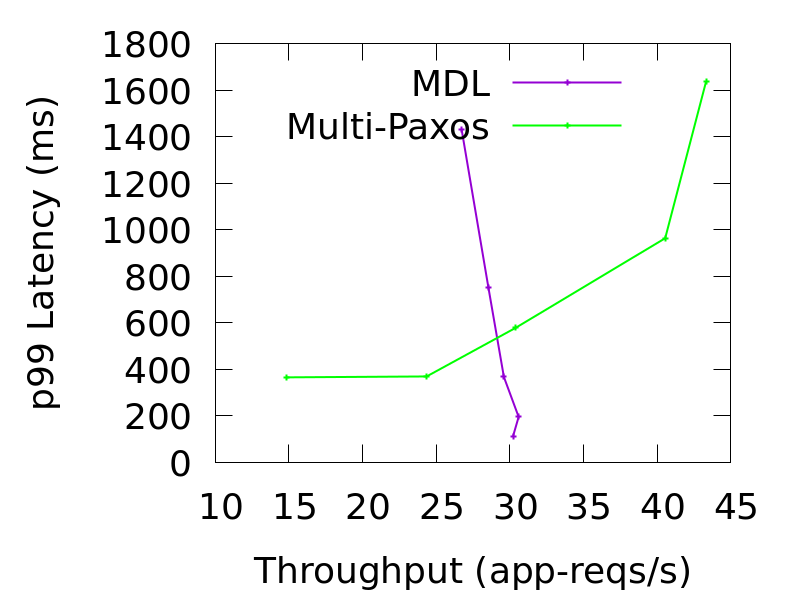
\includegraphics[scale=.15]{figs/1sh_f1000_p99.png}
  \label{fig:1shardp99last}
}
\caption{p99 for single shard setting.}
\end{figure*}
%%%%%%%%%%%%%%%%%%%%%%%%%%%%%%%%%%%%%%%%%%%%%%%%%%%%%%%%%%%%%%%%%%%%%%%%%%%%%%%%%%%
%%%%%%%%%%%%%%%%%%%%%%%%%%%%%%%%%%%%%%%%%%%%%%%%%%%%%%%%%%%%%%%%%%%%%%%%%%%%%%%%%%%

Figures~\ref{fig:1shardp99first}--\ref{fig:1shardp99last} compare the p99
end-to-end application request latency and throughput for \system{} and \mpaxos{}
configured with a single shard with a uniform key distribution and fanouts from
$1$ to $1000$.

\system{} has lower latency than \mpaxos{} when fanout is larger than $1$---over 2x
faster at fanouts $100$ and $1000$---but, in general, performs sub-optimally due
to unnecessary coordination requests. While a protocol that provides \mdl could
be optimized for a single-shard setting~\cite{ongaro2014consensus}, we only evaluate
our multi-sharded protocol and, therefore, still issue coordination messages for
each request.

In particular, when the leader is under high load at higher fanouts, higher load
and must process a large log of buffered requests and each of their coordination
messages. Lower latency is attenuated by the processing of coordination overhead
for each request. While not shown, this improvement is even greater for p90 and
p50, where the tail variability of subrequest latency is less pronounced.

Techniques such as batching could be employed to reduce the number of messages
sent for each request. For example, the final agreement messages sent after a
request is coordinated and committed could be amortized across multiple entries
ordered in the log. Such techniques would increase the maximum throughput of
\protocol while maintaining gains in end-to-end latency.

\subsection{Multi-Shard}
\label{sec:shards}
% %%%%%%%%%%%%%%%%%%%%%%%%%%%%%%%%%%%%%%%%
% %%%%%%%% 3 shard uniform p99 %%%%%%%%%%%
% %%%%%%%%%%%%%%%%%%%%%%%%%%%%%%%%%%%%%%%%
% \begin{figure*}[tbp]
% \centering
% \subfloat[Fanout\xspace1]{
%   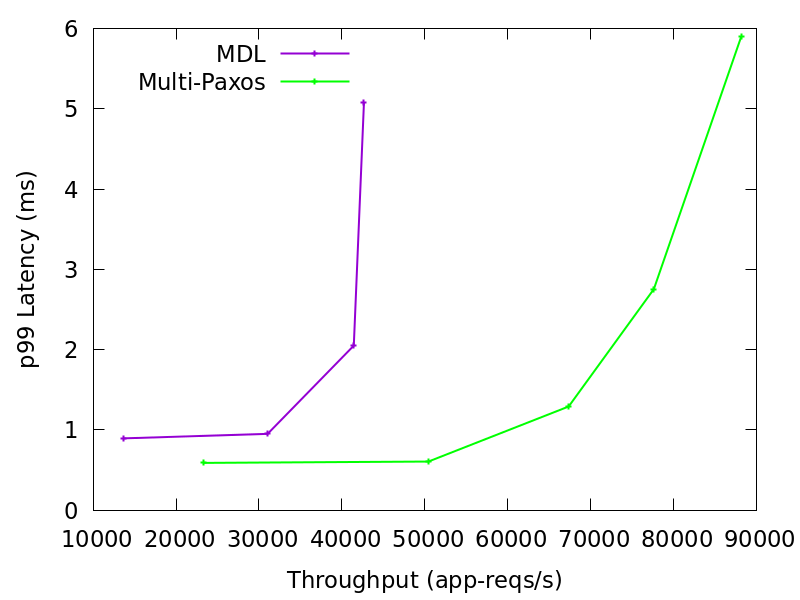
\includegraphics[scale=.15]{figs/3sh_f1_p99.png}
%   \label{fig:3shardp99first}
% }
% \subfloat[Fanout\xspace10]{
%   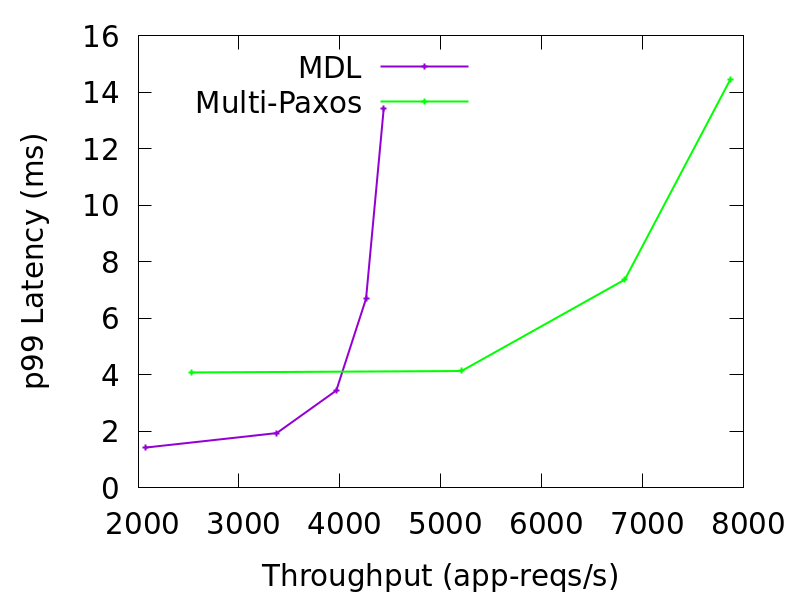
\includegraphics[scale=.15]{figs/3sh_f10_p99.png}
% }
% %\hspace{0mm}
% \subfloat[Fanout\xspace100]{
%   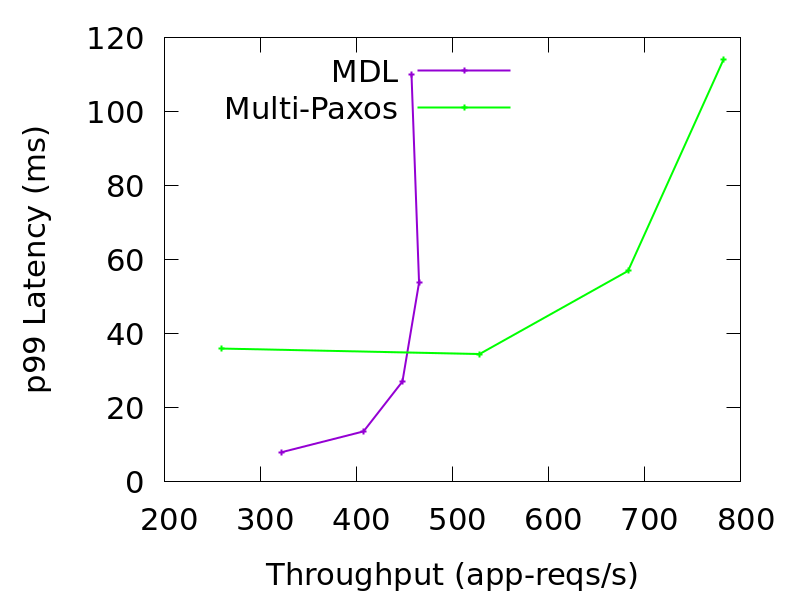
\includegraphics[scale=.15]{figs/3sh_f100_p99.png}
% }
% \subfloat[Fanout\xspace1000]{
%   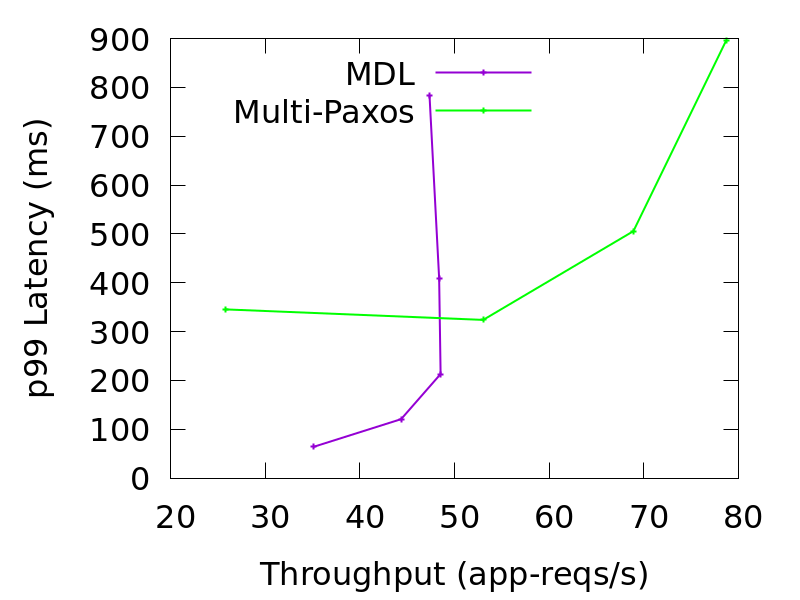
\includegraphics[scale=.15]{figs/3sh_f1000_p99.png}
%   \label{fig:3shardp99last}
% }
% \caption{p99 for 3 shard setting.}
% \end{figure*}
%%%%%%%%%%%%%%%%%%%%%%%%%%%%%%%%%%%%%%%%
%%%%%%%% 9 shard uniform p99 %%%%%%%%%%%
%%%%%%%%%%%%%%%%%%%%%%%%%%%%%%%%%%%%%%%%
\begin{figure*}[tbp]
\centering
\subfloat[Fanout\xspace1]{
  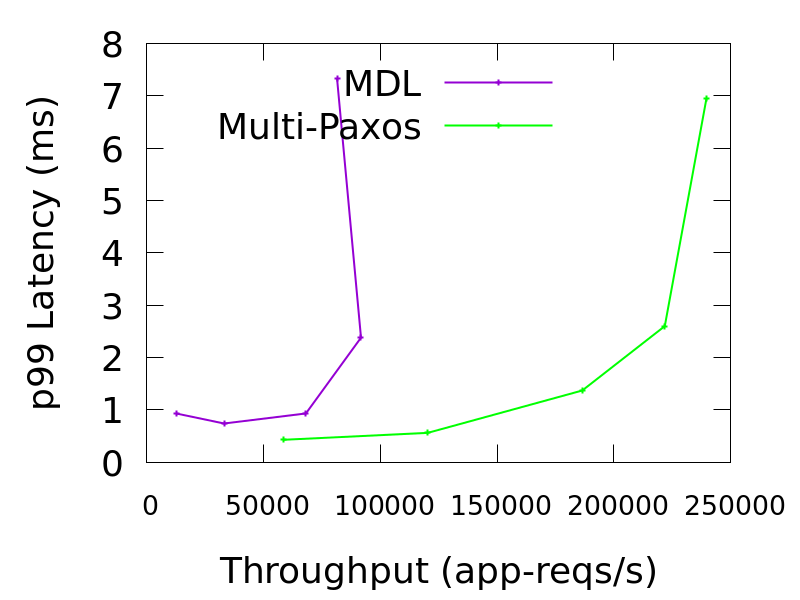
\includegraphics[scale=.15]{figs/9sh_f1_p99.png}
  \label{fig:9shardp99first}
}
\subfloat[Fanout\xspace10]{
  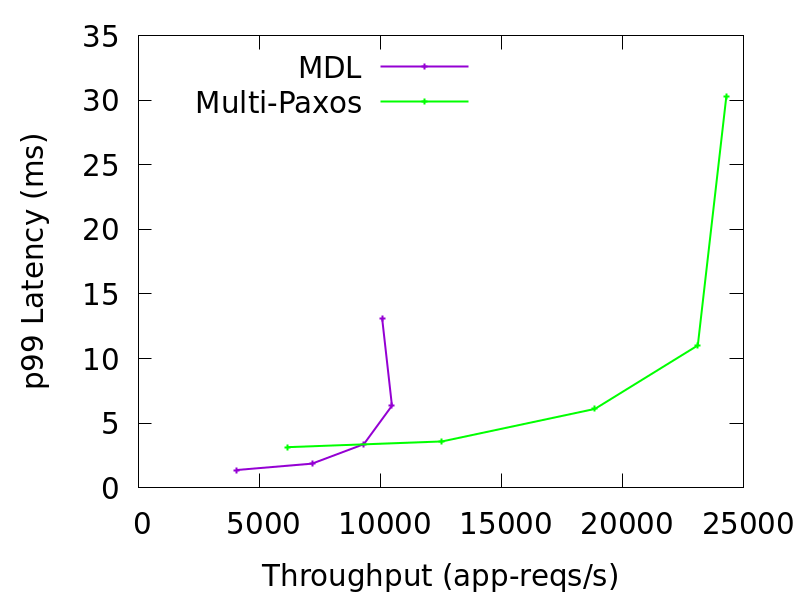
\includegraphics[scale=.15]{figs/9sh_f10_p99.png}
}
%\hspace{0mm}
\subfloat[Fanout\xspace100]{
  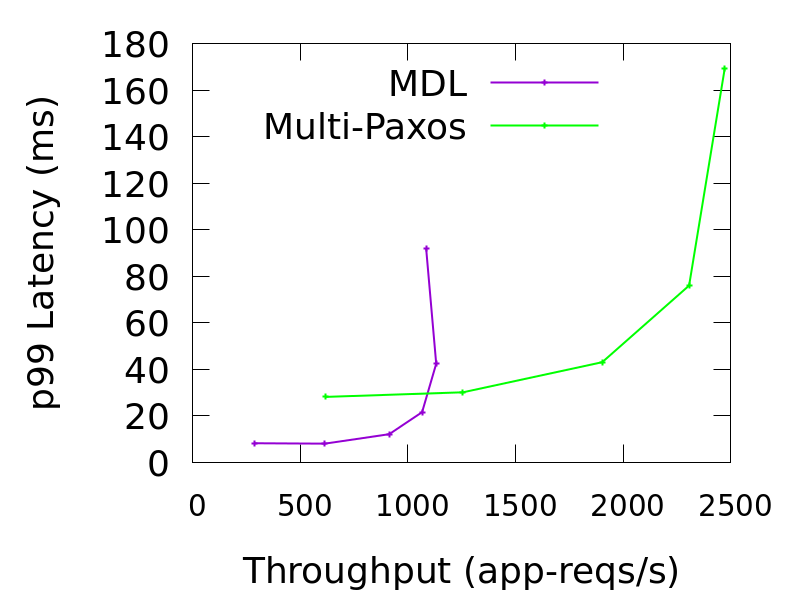
\includegraphics[scale=.15]{figs/9sh_f100_p99.png}
}
\subfloat[Fanout\xspace1000]{
  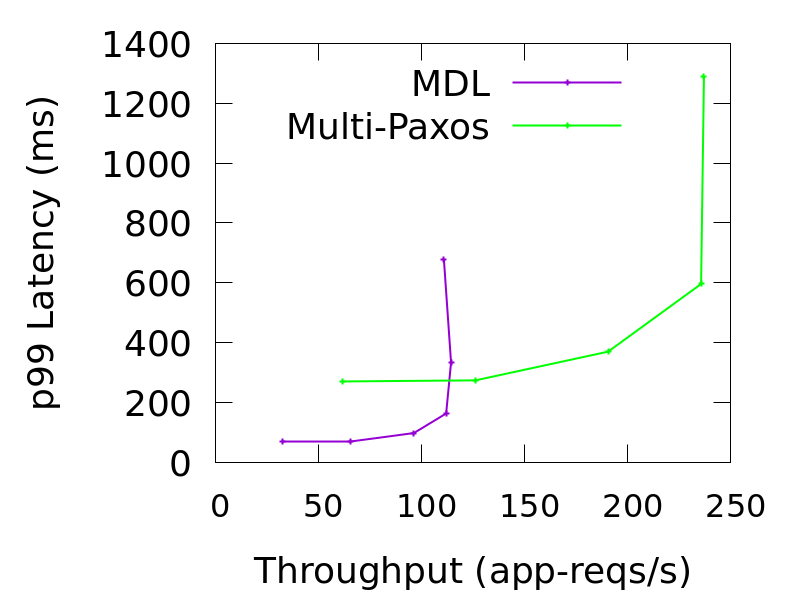
\includegraphics[scale=.15]{figs/9sh_f1000_p99.png}
  \label{fig:9shardp99last}
}
\caption{p99 for 9 shard setting.}
\end{figure*}
%%%%%%%%%%%%%%%%%%%%%%%%%%%%%%%%%%%%%%%%%%%%%%%%%%%%%%%%%%%%%%%%%%%%%%%%%%%%%%%%%%%
%%%%%%%%%%%%%%%%%%%%%%%%%%%%%%%%%%%%%%%%%%%%%%%%%%%%%%%%%%%%%%%%%%%%%%%%%%%%%%%%%%%

% \Crefrange{fig:3shardp99first}{fig:3shardp99last}
% and~\ref{fig:9shardp99first}--\ref{fig:9shardp99last} show p99 latencies and
% throughput for 3-shard and 9-shard configurations, respectively.

\Crefrange{fig:9shardp99first}{fig:9shardp99last}
show p99 latencies and
throughput for a 9-shard configurations.
(Figures for a 3-shard configuration are similar and are omitted due to space constraints.)

%Somewhat counter-intuitively, three shards outperforms nine. 
Similar to
the single-shard case, with fewer shards, the average leader-leader
coordination latency is lower, as fewer operations coordinate across leaders.
This is attenuated by higher per-shard load, as in the single-shard case.

The nine-shard configuration approaches the lower bound improvement
described in \cref{sec:design} for fanouts $100$ and $1000$, with p99 latency
close to 25\% of \mpaxos{}.  An application-level request of fanout $n$ induces
$n-1$ 1-way inter-shard coordination messages that must be serialized with
predecessor fault-tolerance and coordination. On the other hand, load balancing
of large number of requests across multiple shards helps speed the processing
time at each leader.

\subsection{Skew}
% %%%%%%%%%%%%%%%%%%%%%%%%%%%%%%%%%%%%%%%%
% %%%%%%%%%%%% 3 shard skew %%%%%%%%%%%%%%
% %%%%%%%%%%%%%%%%%%%%%%%%%%%%%%%%%%%%%%%%
% \begin{figure*}[tbp]
% \centering
% \subfloat[skew\xspace0.5]{
%   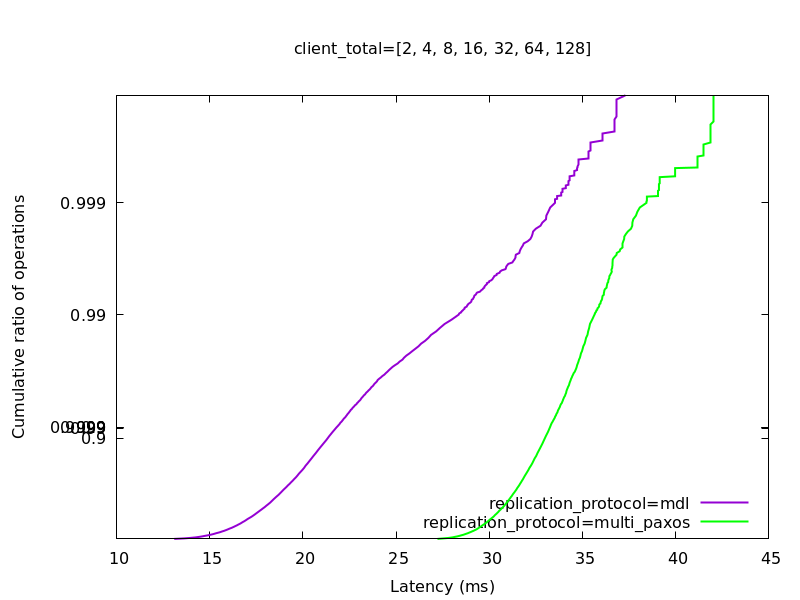
\includegraphics[scale=.2]{figs/3shards_fanout100_skew0.5_8client_CDF.png}
%   \label{fig:3shardsskew}
% }
% \subfloat[skew\xspace0.9]{
%   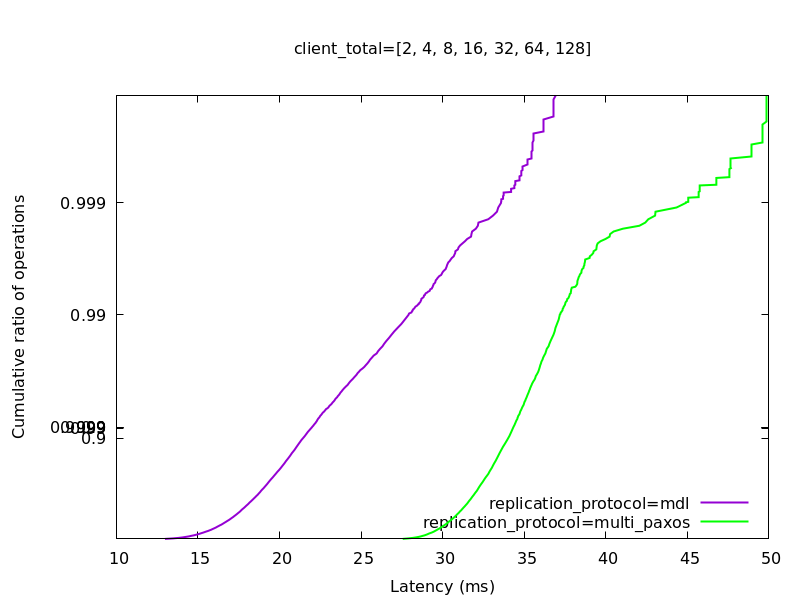
\includegraphics[scale=.2]{figs/3shards_fanout100_skew0.9_8client_CDF.png}
% }
% \subfloat[skew\xspace1.3]{
%   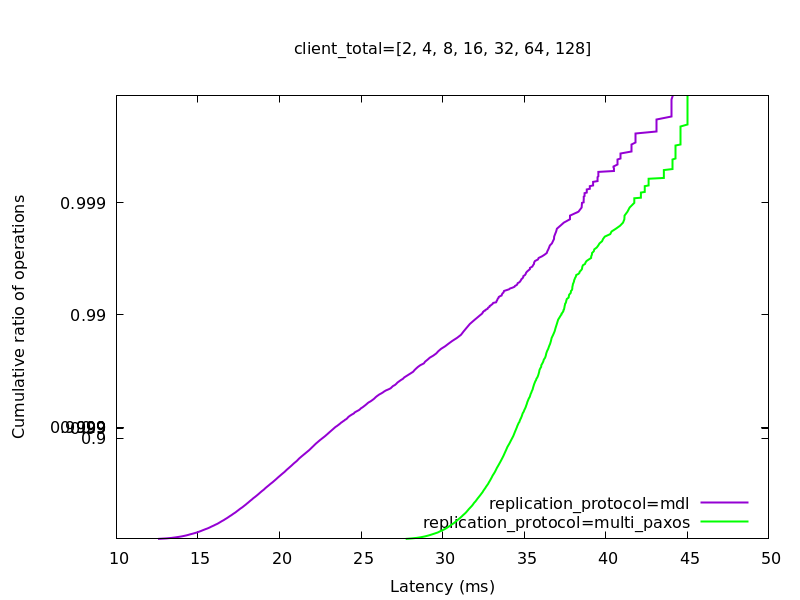
\includegraphics[scale=.2]{figs/3shards_fanout100_skew1.3_8client_CDF.png}
%   \label{fig:3shardsskewlast}
% }
% \caption{3 shard skew.}
% \end{figure*}


%%%%%%%%%%%%%%%%%%%%%%%%%%%%%%%%%%%%%%%%
%%%%%%%%%%%% 9 shard skew %%%%%%%%%%%%%%
%%%%%%%%%%%%%%%%%%%%%%%%%%%%%%%%%%%%%%%%
\begin{figure*}[tbp]
\centering
\subfloat[skew\xspace0.5]{
  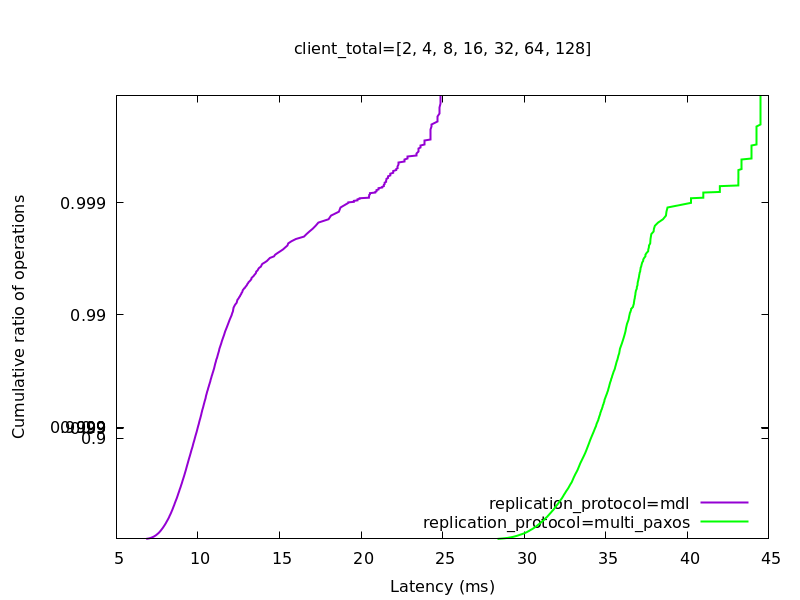
\includegraphics[scale=.2]{figs/9shards_fanout100_skew0.5_8client_CDF.png}
  \label{fig:9shardsskew}
}
\subfloat[skew\xspace0.9]{
  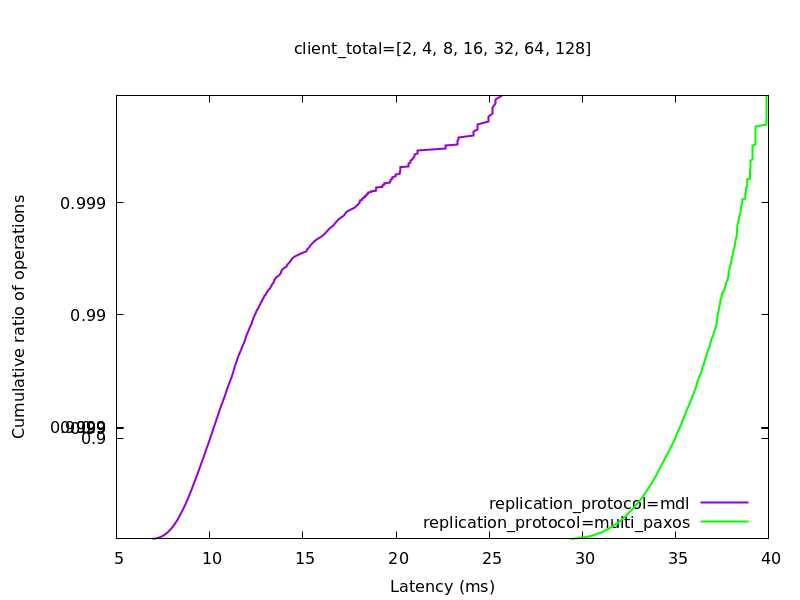
\includegraphics[scale=.2]{figs/9shards_fanout100_skew0.9_8client_CDF.png}
}
\subfloat[skew\xspace1.3]{
  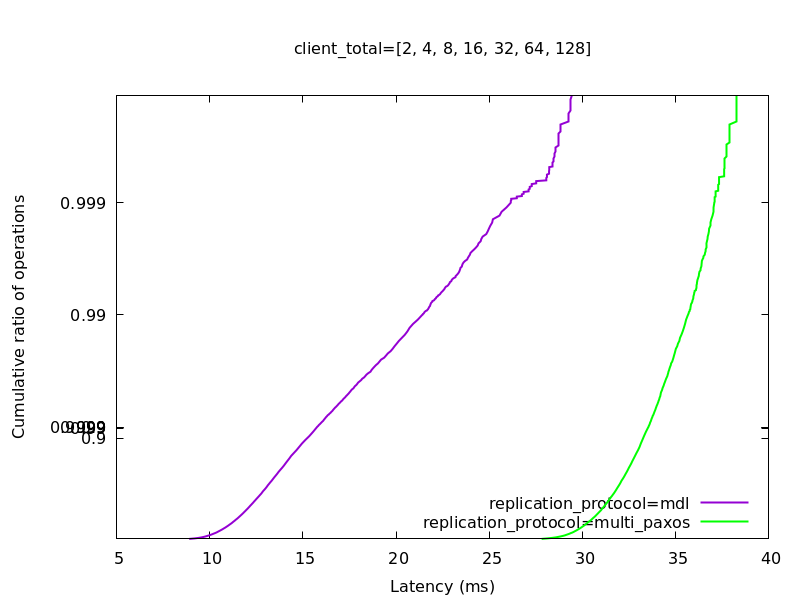
\includegraphics[scale=.2]{figs/9shards_fanout100_skew1.3_8client_CDF.png}
  \label{fig:9shardsskewlast}
}
\caption{9 shard skew.}
\end{figure*}

%%%%%%%%%%%%%%%%%%%%%%%%%%%%%%%%%%%%%%%%%%%%%%%%%%%%%%%%%%%%%%%%%%%%%%%%%%%%%%%%%%%
%%%%%%%%%%%%%%%%%%%%%%%%%%%%%%%%%%%%%%%%%%%%%%%%%%%%%%%%%%%%%%%%%%%%%%%%%%%%%%%%%%%
%%%%%%%%%%%%%%%%%%%%%%%%%%%%%%%%%%%%%%%%%%%%%%%%%%%%%%%%%%%%%%%%%%%%%%%%%%%%%%%%%%%

% \Crefrange{fig:3shardsskew}{fig:3shardsskewlast} and
% ~\ref{fig:9shardsskew}--\ref{fig:9shardsskewlast} show various skew values for
% the 3-shard and 9-shard configurations. 

\Crefrange{fig:9shardsskew}{fig:9shardsskewlast} and
show various skew values for
the 9-shard configurations. 
(Figures for a 3-shard configuration are similar and are omitted due to space constraints.)


We generate keys according to a Zipfian
distribution with varying skew values $\theta \in \{0.5, 0.9, 1.3\}$,
and use a keyspace of size 1 million. We look at CDFs for application-level
requests with fanout 100 issued by 8 concurrent clients.

Increasingly higher skew approaches single shard performance, where \system's
coordination is cheaper, as it does not include network latency, but experiences
overload sooner.  Overall skew has little impact on end-to-end latency until a
high skew value of 1.3, where the tail latency for application-level requests
starts increasing at lower percentiles, by about 2x. We notice this degradation
begin earlier at around skew 1.1 as well. We expect much of this is due to the
high load on the leader responsible for highly contentious keys.

\begin{comment}
\subsection{MDL with Geo-rep in the Wide Area}
\label{sec:wide}
We show the e2e app. latency for varying inter-shard latency (which we call the wide area **this might be wrong terminology) and inter-replica latency (which we call geo-replication, also might be wrong terminology).

\subsection{Applications on MDL}
\label{sec:apps}

As described in prior sections, we built a tool to automatically transform applications built to interact with SDL backends to interact with MDL backends, maintaining external equivalence. In this section we select 3 representative applications, A1, A2, A3, and show that when transformed with our tool, all 3 see an improvement in e2e latency. We use DeathStar to benchmark the applications.

A1 is an application that ....

A2 is an application that ...

A3 is an application that ...

We expect transformed applications that have a large degree of data parallelism and are read heavy running on MDL backends to see the largest e2e latency improvements over their pre-transformed counterparts running on SDL backends.

Jeff is still looking for these applications at the moment -- it would be good to pick applications that are read heavy and some that are mixed. All should include varying degrees of data parallelism, to show how some improve after the transformation more than others.
\end{comment}
